\documentclass[10pt,a4paper]{article}
\usepackage[utf8]{inputenc}
\usepackage[german]{babel}
\usepackage{mathrsfs}
\usepackage{amsmath}
\usepackage{amsfonts}
\usepackage{amssymb}
\usepackage{amsthm}
\usepackage[left=2cm,right=2cm,top=2cm,bottom=2cm]{geometry}
\usepackage{graphicx}

\begin{document}

\section{Aufgabe 7.1}

\subsection{Teil a}

Hierbei geht man ähnlich vor wie bei dem CYK-Algorithmus selst.
Zuerst sieht man, dass es für die Terminale auf der untersten Ebene der Pyramide immer genau einen Syntaxbaum gibt pro Nichtterminal, das dieses erzeugt.
Man speichert also statt einem Nichtterminal $N$ ein Tupel $(N, n)$, wobei $n$ die Anzahl von Syntaxbäumen ist, die man von dort aus mit Startsymbol $N$ erzeugen und den entsprechenden Teil des Worts ergeben.
Jeder Knoten in der Pyramide ist somit eine Menge von 2-Tupeln.
Wenn man einen neuen Knoten berechnet, berechnet man auch kombinatorisch für die gefundenen Nichtterminale die Anzahl möglicher Syntaxbäume.
Findet man also $(A_{i}, a_{i})$ und $(B_{i}, b_{i})$ beim Durchlauf des CYK-Algorithmus und gibt es eine Regel $C \rightarrow A_{i}B_{i}$ so merke man sich $c_{i} = a_{i}b_{i}$.
Am Ende fügt man dann das Tupel $(C, \sum_{i} c_{i})$ in den Knoten ein.

\subsection{Teil b}

Für den CYK-Algorithmus ersetze man $P$ durch die CNF-Umformung $P'$.
\begin{align*}
  P' = \{ & S \rightarrow SS_{+},\\
  & S_{+} \rightarrow N_{+}S,\\
  & S \rightarrow SS,\\
  & S \rightarrow N_{(}S_{)},\\
  & S_{)} \rightarrow SN_{)},\\
  & S \rightarrow SN_{*},\\
  & S \rightarrow a,\\
  & N_{(} \rightarrow (,\\
  & N_{)} \rightarrow ),\\
  & N_{+} \rightarrow +,\\
  & N_{*} \rightarrow * \}
\end{align*}

In der Zeichnung sind die Tupel eigentlich alle in Mengen, aber ich habe die Klammern weggelassen, wenn es 1-elementige Mengen waren.

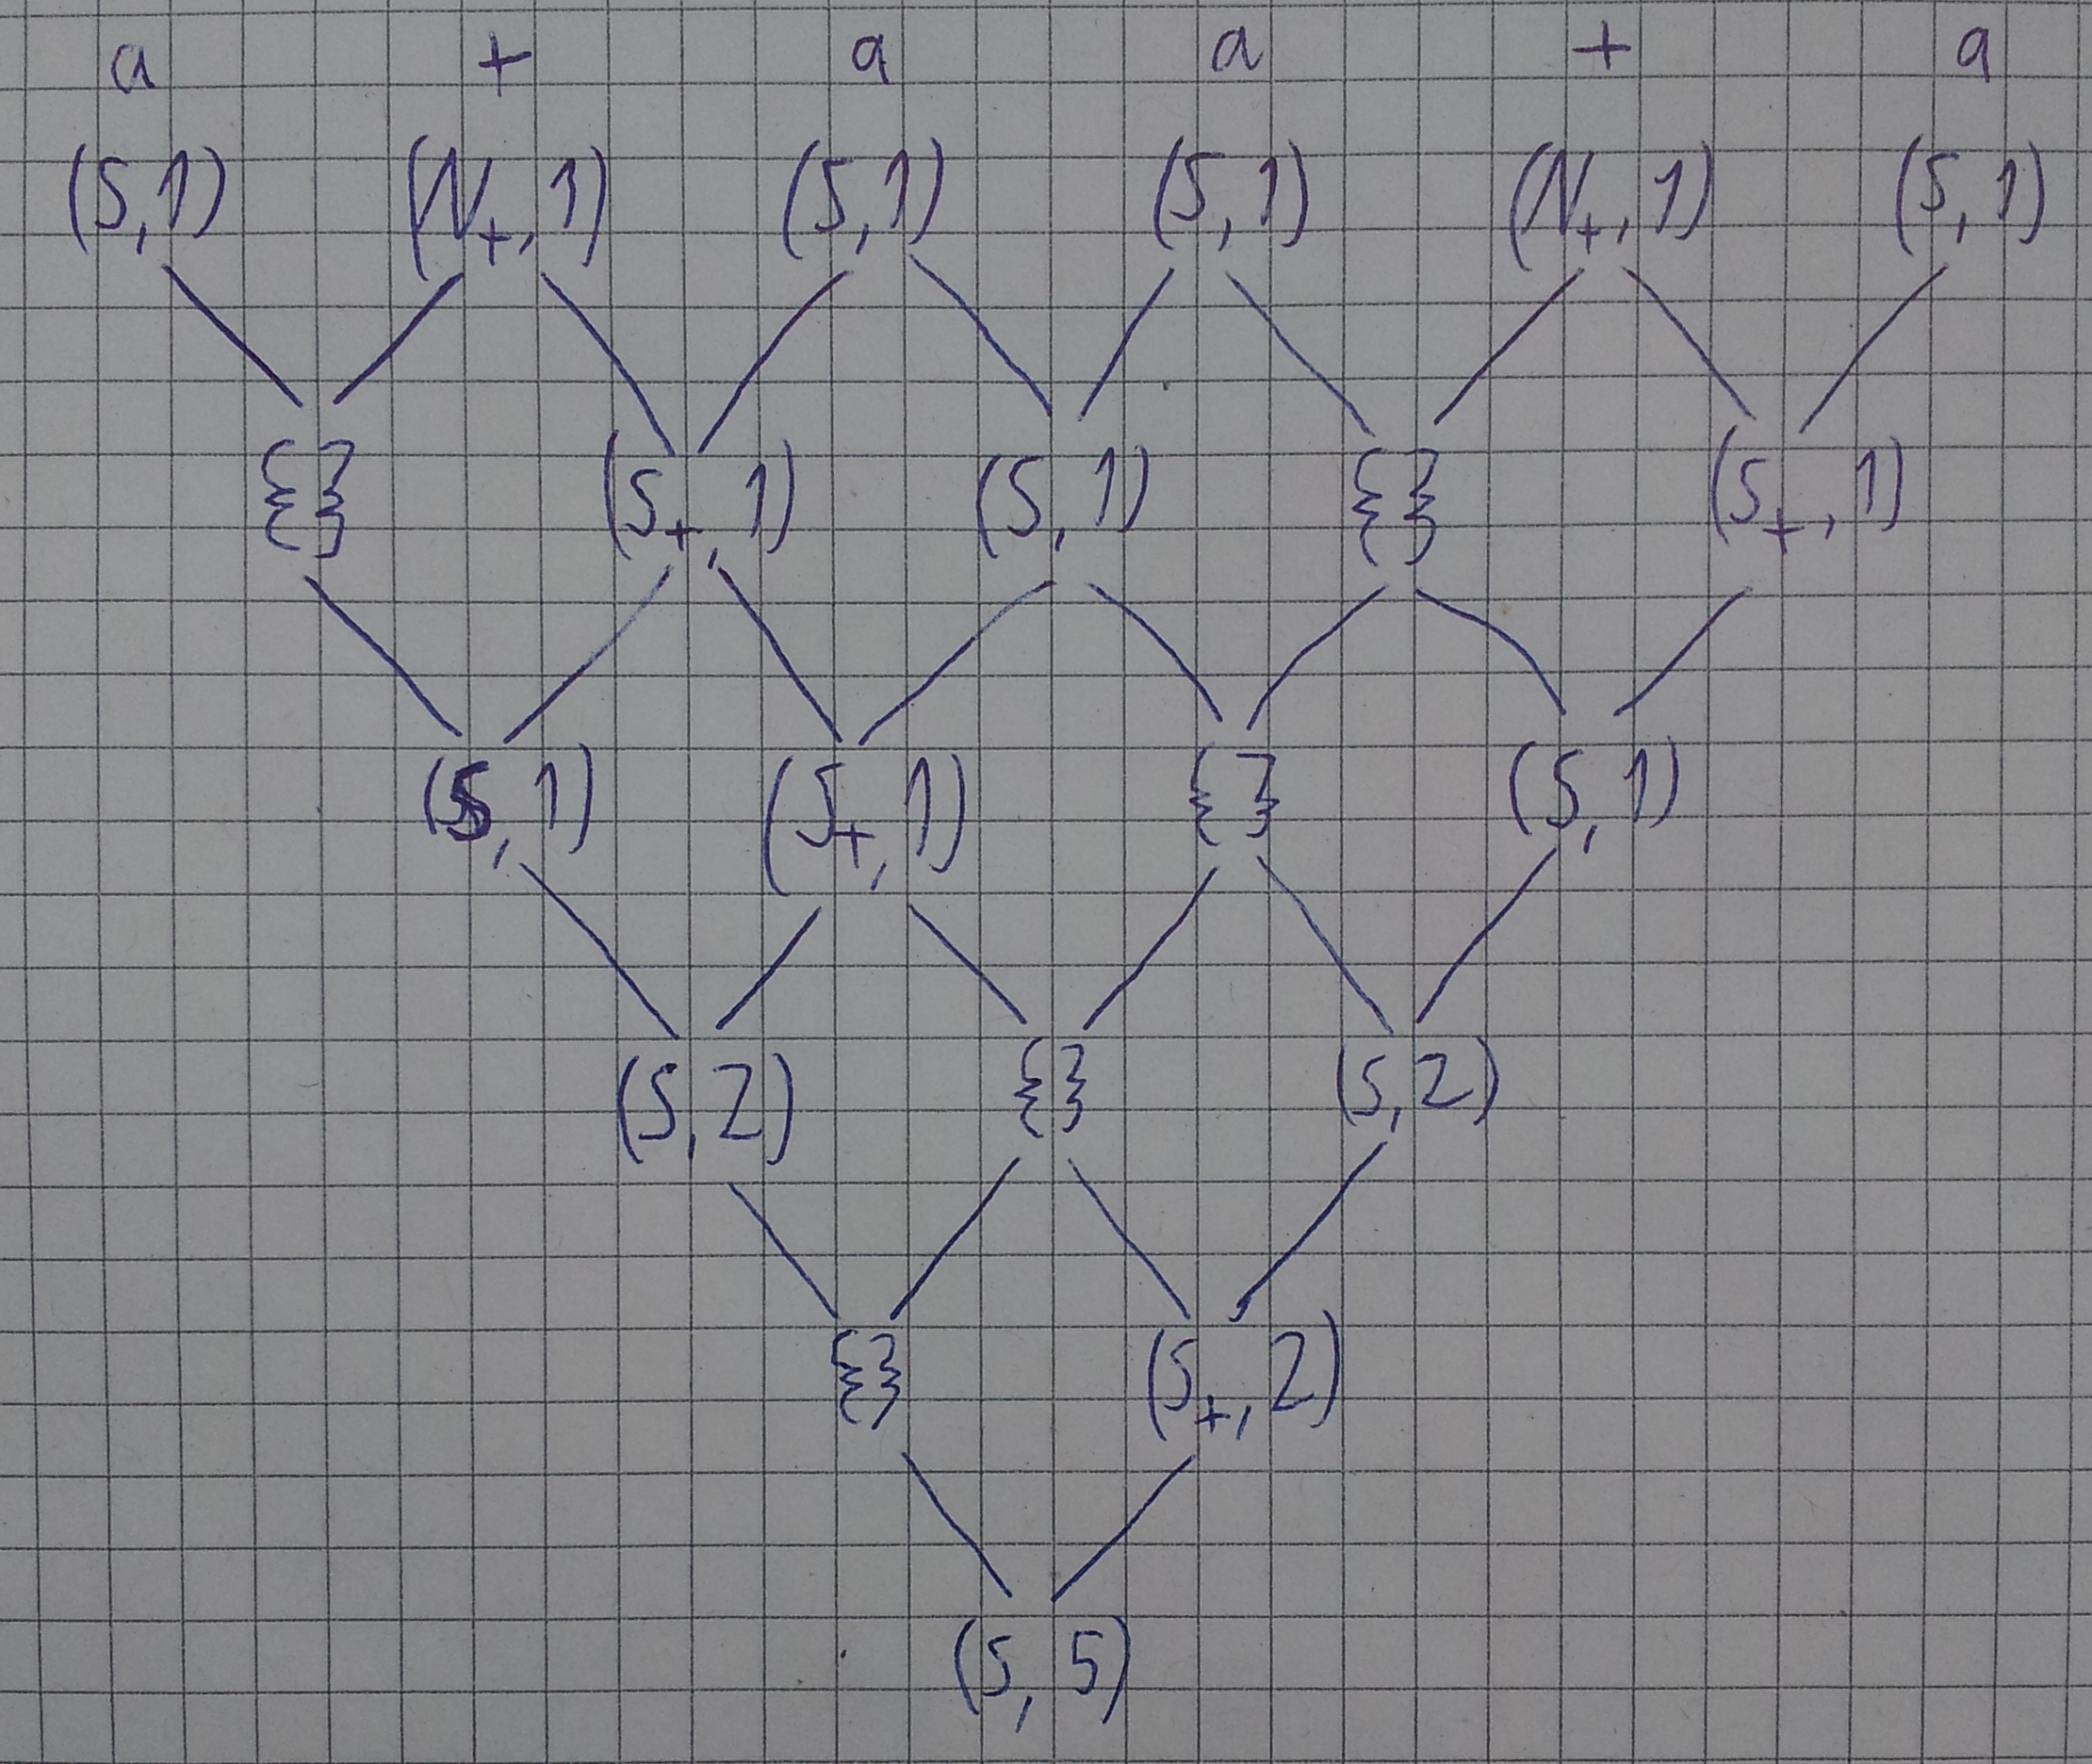
\includegraphics[width=400pt]{7_1_b.png}

Also ist das Wort enthalten und es gibt $5$ verschiedene Syntaxbäume.

\section{Aufgabe 7.2}

\subsection{Teil a}

\begin{align*}
  & (z_{0}, bababb, \#)\\
  & (z_{2}, ababb, B\#)\\
  & (z_{3}, babb, \#)\\
  & (z_{1}, babb, A\#)\\
  & (z_{1}, abb, \#)\\
  & (z_{0}, abb, \#)\\
  & (z_{1}, bb, AA\#)\\
  & (z_{1}, b, A\#)\\
  & (z_{1}, \lambda, \#)\\
  & (z_{0}, \lambda, \#)\\
  & (z_{4}, \lambda, \lambda)\\
\end{align*}

\subsection{Teil b}

\subsubsection{$b^{3}ab^{4}a^{3}$}

Der Keller enthält nur $\#$.

\subsubsection{$a^{2}b^{3}$}

Der Kellerinhalt ist $A\#$.

\subsection{Teil c}

\begin{equation}
    L(M) = \{ ((X)^{i}(Y | (YZ))^{k})^{j} \}
\end{equation}
mit
\begin{equation}
  X, Y, Z \in \{ a, b \}^{*}
\end{equation}
und
\begin{equation}
  |FIRST_{k}(X)|_{b} = 2|FIRST_{k}(X)|_{a}\ \textit{für $k = [LENGTH(X)]$}
\end{equation}
und
\begin{equation}
  |FIRST_{k}(X)|_{b} \le 2|FIRST_{k}(X)|_{a}  - 1\ \forall k \in [1, \dots, LENGTH(X) - 1]
\end{equation}
und
\begin{equation}
  |FIRST_{k}(Y)|_{b} = 2|FIRST_{k}(X)|_{a}\ \textit{für $k = [LENGTH(X)]$}
\end{equation}

\subsection{Teil d}

$M$ ist nicht-deterministisch, weil man im Zustand $z_{0}$ mit $\#$ oben auf dem Stapel entscheiden muss, ob man mit $\lambda$ in $z_{4}$ wechselt oder $a$ oder $b$ liest.

\section{Aufgabe 7.3}

\subsection{Teil a}

Definiere den deterministischen Kellerautomaten $(\{ 0, 1 \}, \{ A, \# \}, \{ z_{0}, z_{1}, z_{2}, z_{3}, z_{4} \}, \delta, z_{0}, \#, \{ z_{0}, z_{3} \})$ mit folgenden Regeln für $\delta$:
\begin{align*}
  & z_{0}0\# \rightarrow z_{1}\#\\
  & z_{0}1\# \rightarrow z_{3}\#\\
  & z_{1}0\# \rightarrow z_{1}A\#\\
  & z_{1}1\# \rightarrow z_{3}\#\\
  & z_{1}0A \rightarrow z_{1}AA\\
  & z_{1}1A \rightarrow z_{2}\lambda\\
  & z_{2}0\# \rightarrow z_{3}\#\\
  & z_{2}1\# \rightarrow z_{3}\#\\
  & z_{2}0A \rightarrow z_{4}\#\\
  & z_{2}1A \rightarrow z_{2}\lambda\\
  & z_{3}0\# \rightarrow z_{4}\#\\
  & z_{3}1\# \rightarrow z_{3}\#\\
  & z_{4}0\# \rightarrow z_{4}\#\\
  & z_{4}1\# \rightarrow z_{4}\#\\
  & z_{4}0A \rightarrow z_{4}\#\\
  & z_{4}1A \rightarrow z_{4}\#
\end{align*}

\subsection{Teil b}

Definiere den deterministischen Kellerautomaten $(\{ 0, 1 \}, \{ \# \}, \{ z_{0} \}, \delta, z_{0}, \#, \{ z_{0}, z_{1}, z_{2} \})$ mit folgenden Regeln für $\delta$:
\begin{align*}
  & z_{0}0\# \rightarrow z_{1}\#\\
  & z_{0}1\# \rightarrow z_{3}\#\\
  & z_{1}0\# \rightarrow z_{1}A\#\\
  & z_{1}1\# \rightarrow z_{2}\#\\
  & z_{1}0A \rightarrow z_{1}AA\\
  & z_{1}1A \rightarrow z_{2}\lambda\\
  & z_{2}0\# \rightarrow z_{3}\#\\
  & z_{2}1\# \rightarrow z_{3}\#\\
  & z_{2}0A \rightarrow z_{3}\#\\
  & z_{2}1A \rightarrow z_{2}\lambda\\
  & z_{3}0\# \rightarrow z_{3}\#\\
  & z_{3}1\# \rightarrow z_{3}\#\\
\end{align*}

\section{Aufgabe 7.4}

\subsection{Teil a}

$G_{1} \in LR(0)$.

\begin{proof}
  Seien $P_{1}, P'_{1}, P_{2}, P'_{2} \in (N \cup E)^{*}$ mit $Q = P_{1}P_{2} = P'_{1}P'_{2} \in L(G_{1})$ und $X, X'$ sodass das die entsprechenden Ableitungen sind.
  Sei $w$ das letzte Terminal von $Q$.
  Dann ist entweder $w = b$ und $X = X' = A$ oder $w = c$ und $X = X' = B$ oder $w = A$ und $X = X' = A$ oder $w = B$ und $X = X' = B$.
\end{proof}

\subsection{Teil b}

$G_{2} \not\in LR(k) \forall k$.

\begin{proof}
  Angenommen $G_{2} \in LR(k)$ für ein $k$.
  Man betrachte die Worte $da^{k}b$ und $da^{k}c$ mit $P_{1} = P'_{1} = \lambda$, $X, X' \in N$, $P_{2}, P'_{2} = d$, $P_{3} = a^{k}b$ und $P'_{3} = a^{k}c$.
  Dann sind $P_{1}P_{2}P_{3}, P'_{1}P'_{2}P'_{3} \in L(G_{2})$ und die ersten $k$ Terminale von $P_{3}$ und $P'_{3}$ stimmen überein, aber $X = A$ und $X' = B$.
\end{proof}

\subsection{Teil c}

$G_{3} \in LR(1)$.

\begin{proof}
  Seien $P_{1}, P_{1}', P_{2}, P_{2}', P_{3}, P_{3}'$ so, dass sie dem Lemma genügen, und $X, X' \in N$.
  $P_{3}$ und $P_{3}'$ beginnen mit einem gemeinsamen Terminal.
  Da sie das terminale Suffix nach dem Nichtterminal sind, können sie aber nur 1 Zeichen lang sein und sind somit identisch.
  Da auch die Präfixe identisch sein müssen, muss das erste Zeichen ebenfalls übereinstimmen.
  Die Kombination aus erstem und letztem Zeichen reicht aus, um eindeutig die verwendete Regel für $C$ zu bestimmen und es kann nur genau eine sein.
  Dann ist aber auch bestimmt, welches Nichtterminal $X$ und $X'$ sind, entweder beide $A$ oder beide $B$.

  Es ist nicht in $LR(0)$, weil man das letzte Zeichen betrachten muss.
\end{proof}

\end{document}